\documentclass[a4paper,11pt]{article}
\usepackage[margin=1in]{geometry}
\usepackage[czech]{babel}
\usepackage{amsmath}
\usepackage{csquotes}

% package na vklad obrázků
\usepackage{graphicx}
\usepackage{caption}
\usepackage{subcaption}
\usepackage{stfloats} % opravuje obrázky přes celou stránku
\graphicspath{ {./images/} } % definování složky s obrázky

% zvyšování hloubky obsahu
\setcounter{tocdepth}{4}
\setcounter{secnumdepth}{4}

% citace
\usepackage[
    citestyle=numeric,
    autocite=superscript,
    sorting=none
    ]{biblatex} 
% \usepackage{biblatex}
\addbibresource{literature.bib}

\DeclareCiteCommand{\supercite}[\mkbibsuperscript]
  {\iffieldundef{prenote}
     {}
     {\BibliographyWarning{Ignoring prenote argument}}%
   \iffieldundef{postnote}
     {}
     {\BibliographyWarning{Ignoring postnote argument}}%
   \bibopenbracket}%
  {\usebibmacro{citeindex}%
   \usebibmacro{cite}}
  {\supercitedelim}
  {\bibclosebracket}
  
% definování listings pro vklad kódu
% \usepackage{listings}
% \lstset{language=js}

% abstrakt s větším písmem (https://tex.stackexchange.com/a/366170)
\makeatletter
\renewenvironment{abstract}{%
    \if@twocolumn
      \section*{\abstractname}%
    \else %% <- here I've removed \small
      \begin{center}%
        {\bfseries \Large\abstractname\vspace{\z@}}%  %% <- here I've added \Large
      \end{center}%
      \quotation
    \fi}
    {\if@twocolumn\else\endquotation\fi}
\makeatother

\selectlanguage{czech} % nastavení jazyka
\include{hyphenation} % upřesnění slabik v různých cizích slovech

\begin{document}

\include{titulnistrany}  % povinné strany
\section{Úvod}
Cílem tohoto projektu bylo vytvořit měřící stanici na měření aktualního počasí a následné zobrazení dat pomocí grafů na webové stránce.

\subsection{Výběr projektu}
Toto téma jsme si vybrali, abychom získali zkušenosti s vytvářením projektu, 
který obsahuje propojení hardwaru se sofwarem, konkrétně propojení stanice s backendem a následné zobrazení dat na webové stránce. 

Prvoplánově jsme zamýšleli vytvořit web pro inzerci produktů,
ale tento nápad se nám nezdál ideální, neboť neobsahoval programátorsky zajímavé prvky a nezdál se nám příliš tvůrčí.

\subsection{Původní zadání}
Aplikace bude mít tři části
\begin{enumerate}
    \item operace a vyrobení hardwaru, který bude měřit počasí (teplota, vlhkost, rychlost a směr větru, déšť) hardware bude obsluhovat Arduino, přičemž si čidla vyrobíme sami (rychlost a směr větru, měření deště)
    \item backend - sbírá data o počasí a ukládá je do databáze, backend bude fungovat i jako API pro jine vývojáře na zjištění aktualního počasí
    \item frontend - webová aplikace zobrazující počasí (mapka, na které budou vidět všechny stanice a bude se dát zobrazit podrobnější data o dané stanici).
\end{enumerate}

\section{Hardware}
Při vytváření stanice bylo nejprve potřeba zvolit vhodný micropočítač pro připojení měřicích komponentů. Nakonec jsme vybrali platformu Arduino,
konkrétně model ESP8266WiFi, který nám umožnil, nejen zapojit všechny různé komponenty potřebné pro měření, ale i připojení k internetu.

\begin{figure}[!htb]
   \begin{minipage}{0.48\textwidth}
     \centering
     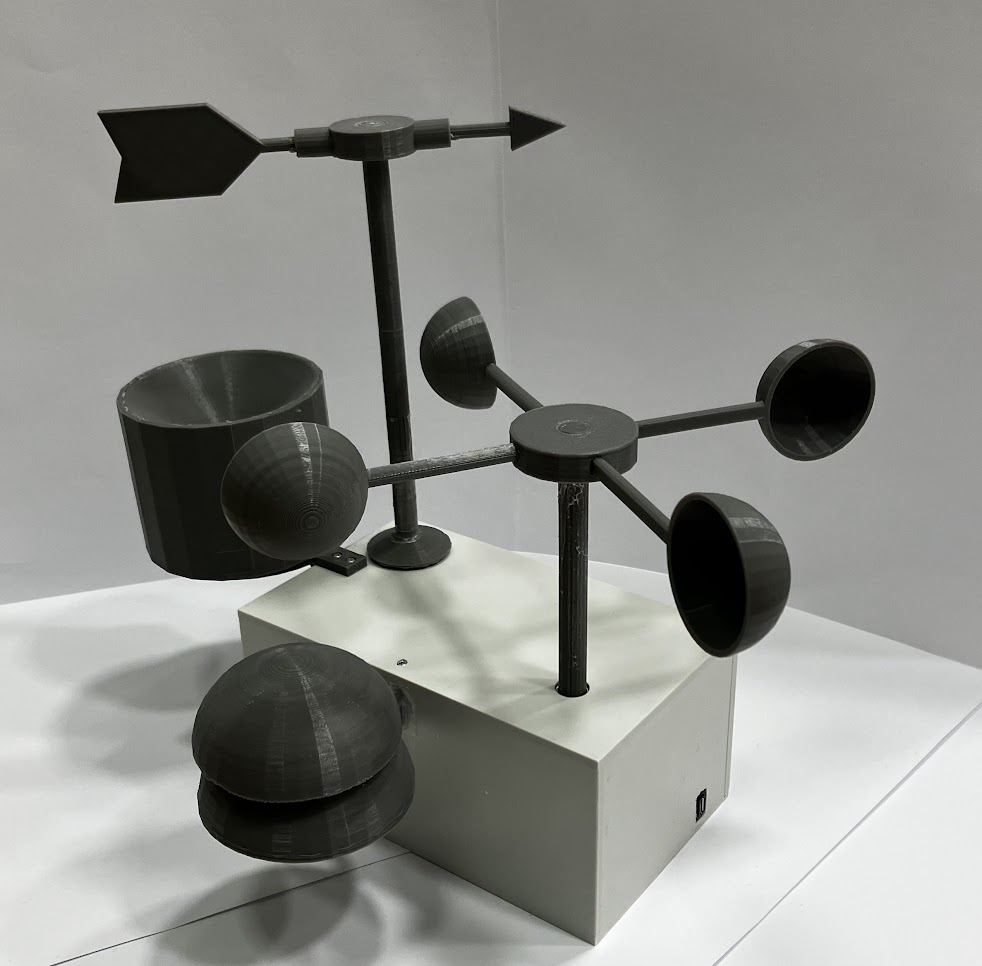
\includegraphics[width=.7\linewidth]{images/stanice0.jpg}
     \caption{Stanice}
   \end{minipage}\hfill
   \begin{minipage}{0.5\textwidth}
     \centering
     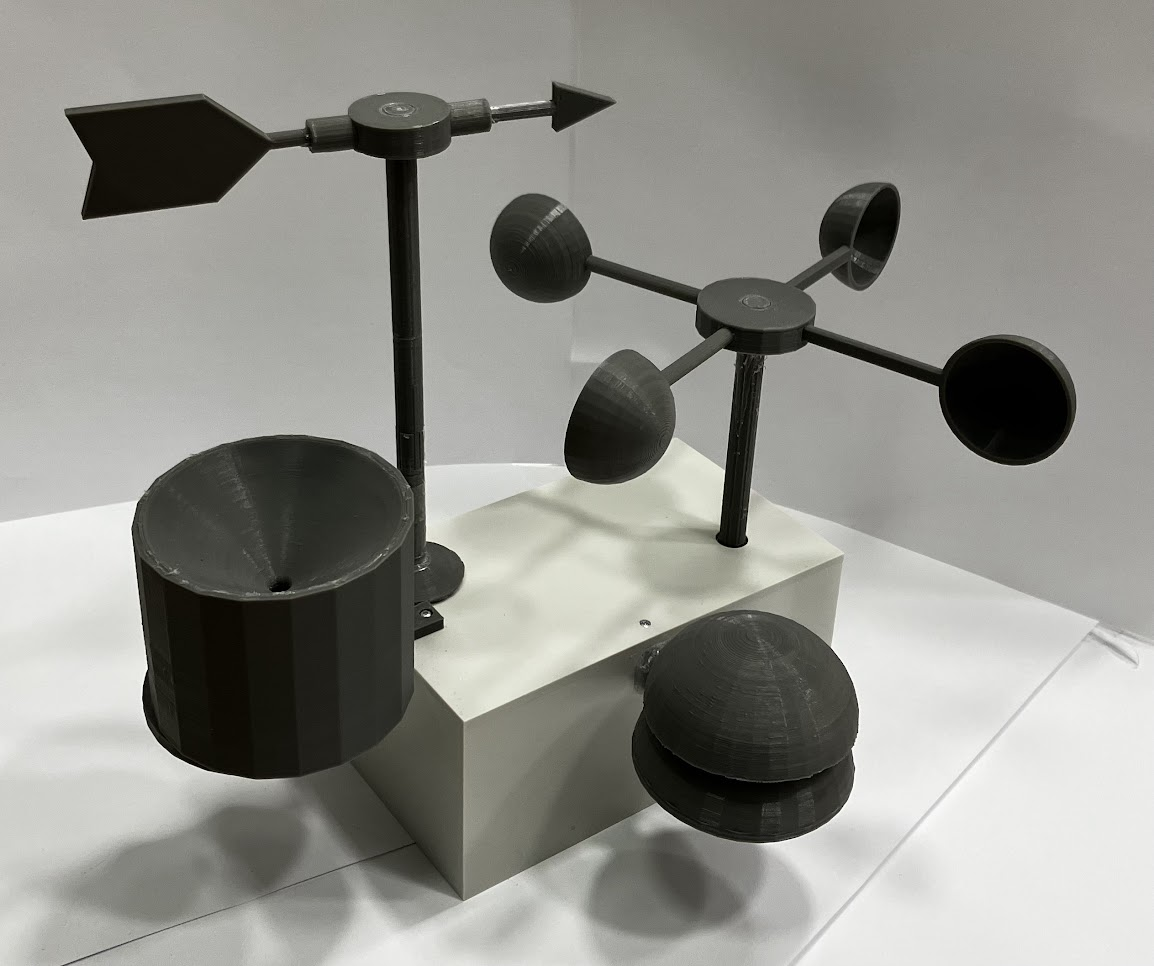
\includegraphics[width=.7\linewidth]{images/stanice1.jpg}
     \caption{Stanice}
   \end{minipage}
\end{figure}
\subsection{Propojení se serverem}
Po zapnutí se stanice připojí k internetu zapomocí Wifi a zaregistruje na backendu (popsáno v kapitole \ref{komunikace}). Jakmile stanice dostane od serveru odpověd s 
JSON Web Tokenem, uloží si ho a při každém opeslání dat na server ho použije k prokázání totožnosti.

\subsection{Měření teploty a vlhkosti}
Pro měření teploty a vlhkosti byl použit Digitální teploměr Adafruit AM2320 Sensor\cite{teplomer}. V případě nebylo zapotřebí vymýšlet jak cokoli měřit,
protože senzor je připojen přes I2C interface, ze kterého program pouze čte již změřené hodnoty.
\begin{figure}[h] 
    \centering
    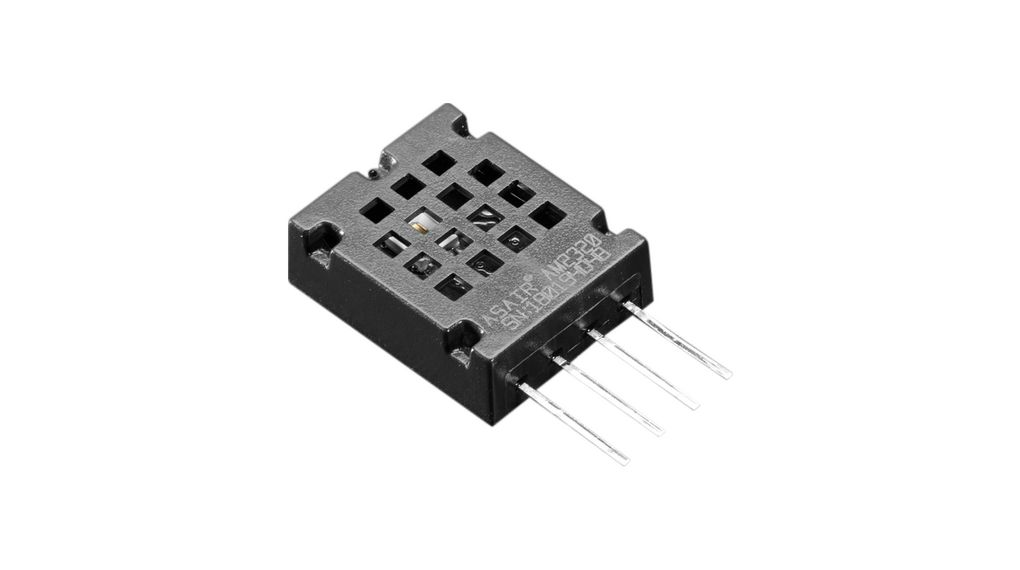
\includegraphics[width=0.25\textwidth]{images/Adafruit-AM2320.jpg}
    \caption{Teploměr a vlhkoměr}
\end{figure}

\subsection{Měření tlaku}
Měření tlaku je zhruba stejně přímočaré jako měření teploty, což znamená, že se o měření stará sensor\cite{tlakoměr},
který zapojen přes I2C interface, ze kterého program čte hodnotu klaku v jednotce Pa.

\begin{figure}[h] 
    \centering
    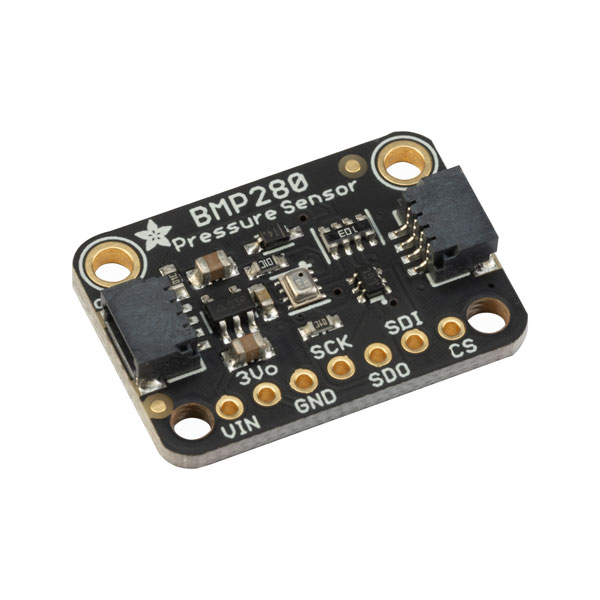
\includegraphics[width=0.25\textwidth]{images/Adafruit-BMP280.jpg}
    \caption{Tlakoměr}
\end{figure}
\subsection{Rychlost větru}
V případě měření rycholsti větru už nestačilo jen koupit sensor, ale bylo potřeba vymyslet jak převést momentum otáčející se osy s lopatkama na realnou rychlost.
Tento problém je vyřešen následujícím způsobem. Na ose je nazen disk kruhovitého tvaru, který má v sobě dírky, skrz které optický senzor vysílá paprsek. Pokud se paprsek přeruší,
znamená to, že se mechanismus otočil o jednu dírku. Program tedy počítá kolikrát se paprsek přeruší a zpočítá skutečnou rychlost větru pomocí následující rovnice.
\begin{equation}
v = n * d / ČasMěření 
\end{equation}
Kde $v$ = rychlost větru, $n$ = počet přerušení, $d$ = vzdálenost uražená větrem na jedno přerušení.

\begin{figure}[h] 
    \centering
    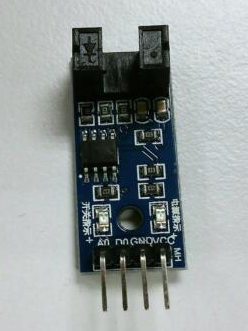
\includegraphics[width=0.25\textwidth]{images/ir_sensor.png}
    \caption{Optická závora}
\end{figure}

\subsection{Směr větru}
Měření směru větru je realizováno pomocí magnetického rotačního senzoru, který dokáže měřit odchylku magnetického pole. To bylo využita na měření odchylky větru tak, že na ose, na které je přidělaná střelka, kterou vítr otáčí, je zespod přidělán
malý magnet a senzro tedy měří jeho odchylku.

\begin{figure}[h] 
    \centering
    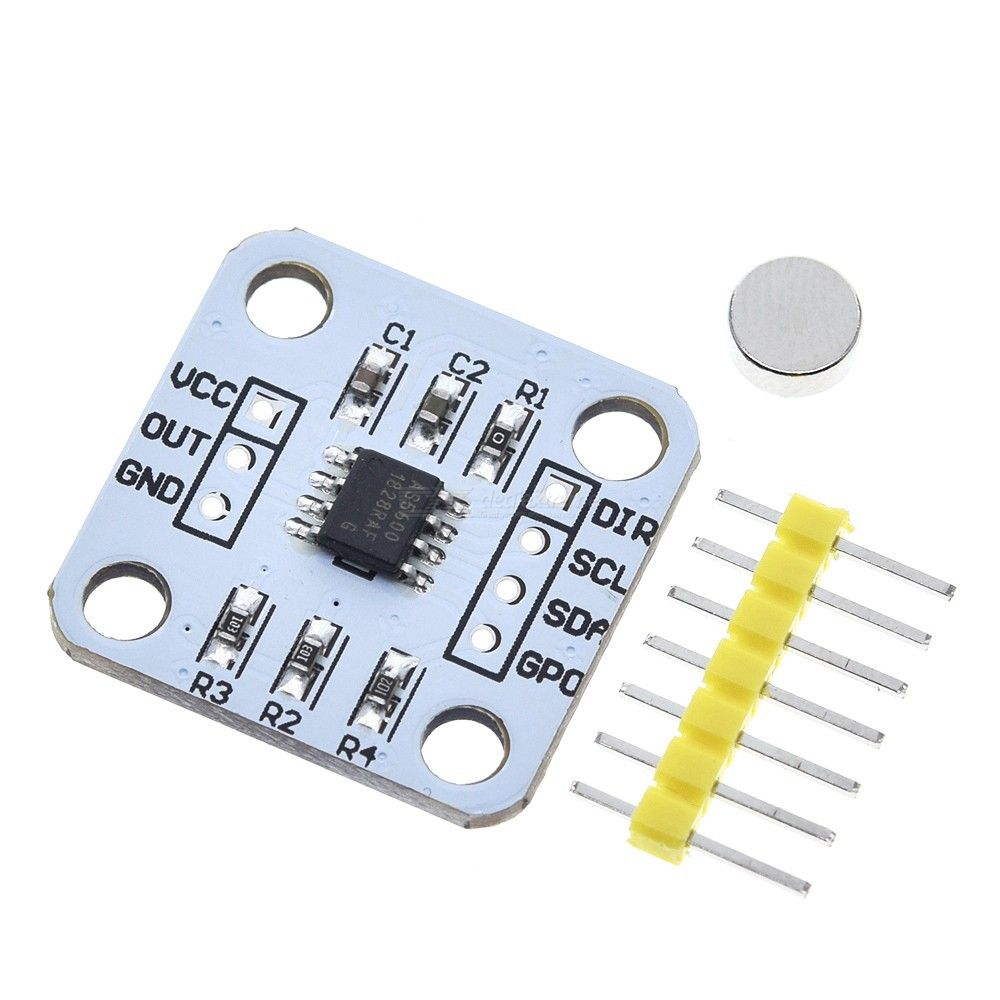
\includegraphics[width=0.25\textwidth]{images/AS5600.jpg}
    \caption{Magnetický rotační sezor}
\end{figure}

\subsection{Měření deště}
Při vytváření součástky na měření deště vzniklo hned několik nápadů jak déšť měřit. Nejprve vznikl nápad, že by skrz trychtýř sbírající vodu prokapávala voda a optický senzor by počítal kapky a tím měřit déšt.
Tento způsob by však nefungoval, protože optický senzor nedokázal rozpoznat padající kapku.

Po delším hledání na internetu jsem však našel řešení\cite{mereni_deste}, které vy tento problém vyřešilo a nebyl by potřeba žádný optický senzor. Toto řešení spočívá v tom, že voda kape to malé kolébky, která se v jeden moment překlopí a voda kape do truhé strany.
Tímto překlopením kolébka zaktivuje senzor rozpoznání magnetického pole, protože na kolébce je přidělán malý magnet.

\begin{figure}[h] 
    \centering
    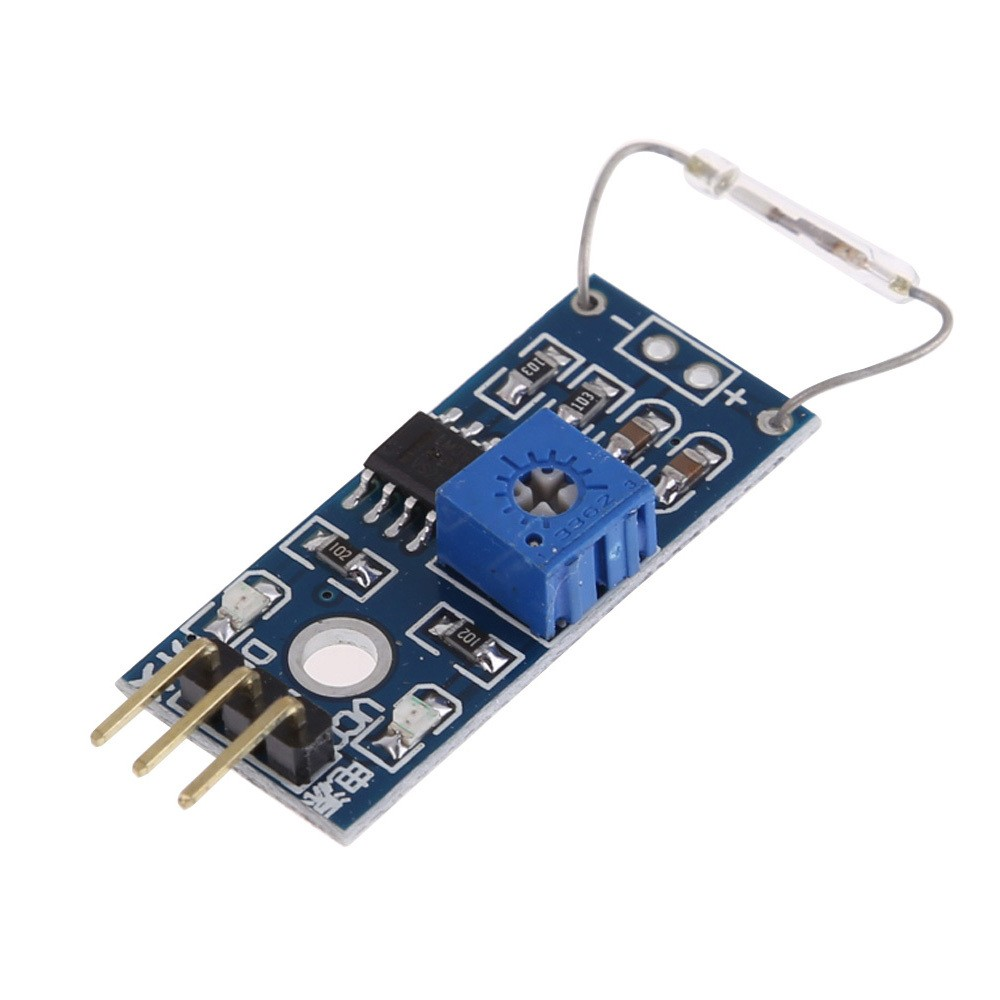
\includegraphics[width=0.25\textwidth]{images/magnet_sensor.jpg}
    \caption{Senzor magnetického pole}
\end{figure}

\subsection{Měření GPS}
Z důvodu, že stanice potřebuje mít informace o své poloze, ve stanice je GPS modul, který získává aktuální GPS souřadnice. Tento senzor má být zapojen na RX/TX piny, ale z důvodu, že na naší arduino desce už
nezbývali volné RX/TX piny, GPS modul musel být zapojen na jiné dva piny a data se z pinů čtou softwarově pomocí knihovny SoftwareSerial. S tímto řešením také ale nastaly první problémy, protože program začal náhodně padat a dlouhou jsem nemohl přijít proč.
Po delším zkoumání jsem přišel na to, že knihovna SoftwareSerial zapisuje data do paměti bezohledu na to, zda je paměť volná, a tudíž začala přepisovat data programu, což způsobilo padání programu.
Tento problém je dosud nevyřešen, protože už nebyl čas na vytvoření vlastní knihovny, která by tento problém řešila. Další možným řešením by bylo použít jinou desku, která by měla více RX/TX pinů, avšak toto řešení už také nebylo možné.

\subsection{Prostor pro zlepšení}
Největším nedostatek je momentálně neúplná funkce GPS modulu, což by do budoucna chtělo nějakým způsobem vyřešit.
Další možnost pro vylepšení by mohlo být přidání kompasu, protože v tento moment je ptřeba natočit stanici správným směrem, aby měřila směr větru přesně. 



\section{Backend}
Backend, neboli serverová část aplikace, našeho projektu slouží primárně k shromažďování a následnému zpracovávání dat. Naše API dále umožňuje bezplatný přístup k těmto datům.
Backend byl vyvinut v Pythonu pomocí knihovny FastApi a pro ukládání dat byla použita databáze PostgreSQL.
Pro odesílání e-mailů byla použita knihovna smtplib a pro komunikaci s platební branou byla použita knihovna stripe. 

Backend může být abstrahován do tří klíčových částí, z nichž každá má specifické úkoly: 
\begin{itemize}
  \item zpřístupnění dat pro Frontend/Developery (pomocí API) 
  \item zajištění komunikace mezi stanicí a databází 
  \item spravování objednávek, objednané prostřednictvím webové stránky (více popsáno v kapitole \ref{frontend})  
\end{itemize}

\subsection{Zpřístupnění dat}
O zpřístupnění naměřených dat se starají veřejné endpointy, které může kdokoli bezplatně použít, ať už pomocí naší webové stránky, či pomocí našeho API. 
V případě použití těchto endpointů, není potřeba žádná autorizace a uživateli vrátí vyžádaná data ve formátu JSON. Mezi tyto veřejné endpointy patří:
\begin{itemize}
  \item GET /stations
  \item GET /now/{gps} 
  \item GET /stats/{gps}
\end{itemize}

První endpoint (/stations) jednoduše vrátí GPS souřadnice všech stanic, které jsou v ten moment zapojené.
Za tímto endpointem se schovává v podstatě jeden SQL dotaz, který z databáze vytáhne všechny aktivní stanice a nakonec funkce vrátí JSON.
\begin{lstlisting}[language=json,firstnumber=1, caption=Příklad požadavku /stations]
{
  "message": "ok",
  "stations": [
    {
      "gps": "50.0993194_14.3596525"
    },
    {
      "gps": "49.7454400_14.0578025"
    }
  ]
}
\end{lstlisting}
Druhý endpoint (/now/{gps}) bere jako parametr GPS souřadnice stanice a podle nich z databáze vytáhne poslední naměřená data dané stanice.
Za tímto endpointem se opět schovává v podstatě jen jeden SQL dotaz, který z databáze vytáhne poslední naměřené hodnoty konkrétní stanice a nakonec funkce vrátí JSON.
\begin{lstlisting}[language=json,firstnumber=1, caption=Příklad požadavku /now/{gps} ]
{
  "message": "ok",
  "time": "24-12-2022 4:20:00",
  "temperature": -3,
  "humidity": 43,
  "pressure": 100000,
  "wind_speed": 13,
  "wind_direction": "N",
  "rain": 4
}
\end{lstlisting}
Poslední endpoint (/stats/{gps}) má za úkol vracet dlouhodobá zprůměrovaná data v časovém rozmezí, které je určeno pomocí query parametrů,
to znamená "date\_from", "date\_to" a nepovinný parametry "freq", který pevně udává frekvenci průměrování dat. Data se průměrují vzhledem k velikosti časového intervalu.
Data v časovém rozmezí, které je menší než tři dny se průměrují po hodině.
Data v časovém rozmezí, které je menší než tři měsíce se průměrují po dnech. Data v rozmezí, které je menší než rok se průměrují po týdnech
a pokud je časové rozmezí větší než rok průměr se dělá z dvou týdnů. Pokud je potřeba průměrovat bez ohledu na velikost časového rozmezí,
stačí nastavit hodnotu parametru query "freq" a data se budou průměrovat vzhledem k hodnotě "freq" následovně:
\begin{itemize}
  \item 1 -> data se průměrují po 5 minutách
  \item 2 -> data se průměrují po 30 minutách
  \item 3 -> data se průměrují po hodině 
  \item 4 -> data se průměrují po dnech 
  \item 5 -> data se průměrují po týdnech 
  \item 6 -> data se průměrují po dvou týdnech 
  \item 7 -> data se průměrují po čtyřech týdnech 
\end{itemize}
O samotném průměrování hodnot se stará samotná databáze pomocí funkce AVG. Celý časový interval se nejprve rozdělí po časových úsecích, které se buď automaticky, nebo podle již zmiňované hodnoty "freq".
Následně se provede SQL dotaz do databáze, který vytáhne zprůměrované hodnoty pro každý časový úsek. Nakonec funkce vrátí tyto hodnoty ve formátu JSON.
\begin{lstlisting}[language=json,firstnumber=1, caption=Příklad požadavku /stats/{gps}]
{
  "message": "ok",
  "data": [
    {
      "time": "1-12-2022 00:00:00",
      "temperature": -3.6,
      "humidity": 41,
      "pressure": 100200,
      "wind_speed": 13,
      "wind_direction": "N",
      "rain": 4,
      "avrage_of": 288
    },
    {
      "time": "2-12-2022 00:00:00",
      "temperature": -2.2,
      "humidity": 49,
      "pressure": 100100,
      "wind_speed": 4,
      "wind_direction": "S",
      "rain": 0,
      "avrage_of": 288
    }
  ]
}
\end{lstlisting}

\subsection{Komunikace se stanicí} \label{komunikace}
Pro komunikaci stanice se serverem stanice využívá dva endpointy:
\begin{itemize}
  \item POST /station/register
  \item POST /station/update
\end{itemize}
V případě prvního endpointu (/station/register) jde primárně o autorizace stanice, aby data na server nemohl posílat neautorizovaný uživatel. Tento POST požadavek očekává v parametru 
sériové číslo stanice a jeho GPS souřadnice. Backend nejprve ověří, zda sériové číslo odpovídá registrovaným stanicím a pokud ano, tak vytvoří JSON Web Token (dále jen JWT),
kterým se stanice dále prokazuje pří dalších interakcích se serverem. Dále si stanici uloží do databáze do seznamu aktivních stanic.

Druhý endpoint (/station/update) slouží k přidání naměřených dat stanicí do databáze. V tomto případě server očekává v hlavičce požadavku již zmiňovaný JWT,
podle kterého server pozná, o jakou jde stanici a naměřená data, která stanice odeslala ve formátu JSON, zapíše do databáze.

\subsection{Správa objednávek}
Celý náš objednávkový systém slouží k tomu, aby si kdokoliv mohl zakoupit naší stanici, čím zajistí, že bude mít možnost měřit počasí kdekoliv bude potřebovat. 
Při vytváření objednávkového systému bylo potřeba nejprve vybrat nějakou platební bránu, která by nám umožnila přijímat platby od zákazníků. V našem případě jsme vybrali platební bránu Stripe.

Pro spravování objednávek backend používá 5 endpointů
\begin{itemize}
  \item POST /payment-webhook
  \item POST /login
  \item GET /orders
  \item GET /order/{id}
  \item POST /update/{id}
\end{itemize}
První endpoint (/payment-webhook) funguje jako webhook\footnote{Webhook je způsob, jakým se automaticky přenášejí data mezi webovými aplikacemi.
Pokud se v jedné aplikaci stane určitá událost, webhook ji zachytí a přenese do druhé aplikace.},
který se zavolá v moment, kdy platební brána vyhodnotí, že objednávka byla zaplacena. V moment kdy se zavolá webhook, do databáze se přidá nová objednávka. 
V ten moment se také odešle zákazníkovi e-mail o tom, že objednávka byla přijata. Zároveň příjde e-mail i adminům s upozorněním, že byla vytvořena nová objednávka.

Endpoint (/login) slouží k autorizaci adminů. Admin se pomocí webové stránky může přihlásit a spravovat jednotlivé objednávky.

Endpoitn (/orders) je endpoint, který vrací ID všech objednávek. Tento endpoint je omezen pouze pro adminy.

Endpoitn (/order/{id}) vrací informace konkrétní objednávky.

Poslední endpoint (/update/{id}) slouží opět jen pro adminy a slouží k upravování stavu objednávky.

\subsection{Databáze}
Backend používa již zmiňovanou databázi PostgreSQL, ve které je pět tabulek zobrazených na obrázku č.\ref{model_databaze}.

\begin{figure}[h] 
    \centering
    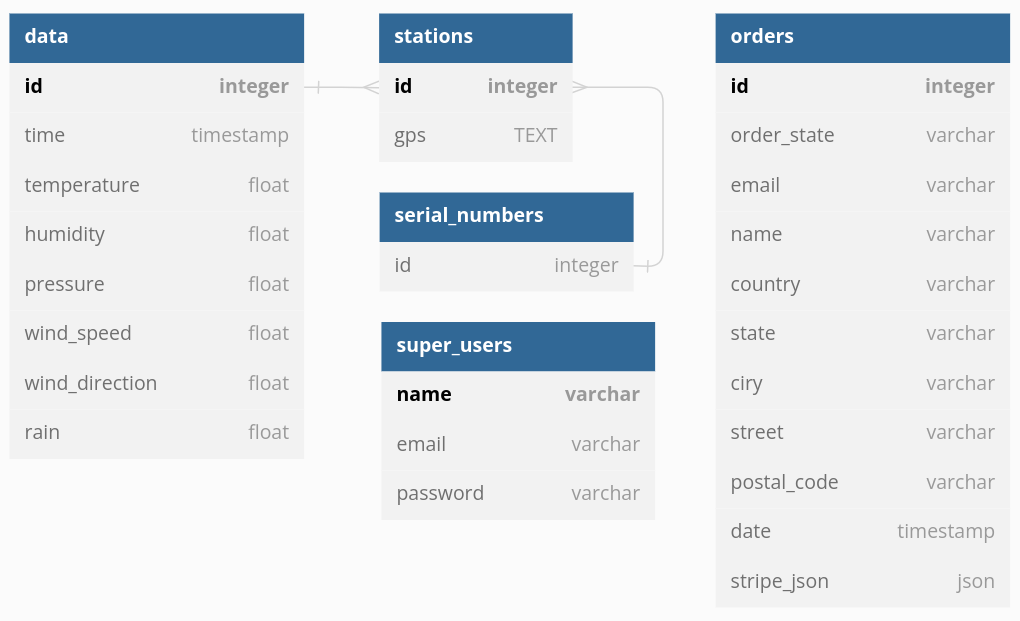
\includegraphics[width=0.7\textwidth]{images/database_diagram.png}
    \caption{Model databáze}
    \label{model_databaze}
\end{figure}

\section{Frontend} \label{frontend}
Frontend slouží jako nástroj pro vizualizaci aplikace. Patří sem veškeré soubory pro vykreslování stránek, obrázky, mapa a grafy. Uživatel může jednoduše přepínat mezi stránky aplikace, kterými jsou: domovská stránka, mapa a údaje o vývojářích.

Frontend aplikace obsahuje soubory vue.js, což je javascriptový framework, který se stará o dynamické a reaktivní zobrazení uživatelského rozhraní. Vue.js je velmi populární a používaná technologie i velkými firmami, která funguje na bázi jednoduchých šablon a komponent.
Vue.js je nováčkem na trhu, ale disponuje rychlostí a velkými možnostmi oproti ostatním frameworkům.
Tato technologie usnadňuje uživatelům jednoduché použití a přehlednou dokumentací. Kvůli rozsáhlému používání jsme usoudili, že vue.js je správná volba. 

Pro odbavování HTTP požadavků jsme použili knihovnu axios, která propojuje backend s frontendem na základě jejich požadavkům. Disponuje rychlostí, jednoduchým odbavováním a odesíláním požadavků a propracovanou dokumentací, která je základem pro správné použití.
Jde o technologii používanou všemi úrovni vývojářů. Aplikace umožňuje odesílání asynchroních požadavků, transformací dat a správou případných chyb.
Za pomocí čtení url stránky posílá axios odpověď. Tímto způsobem se dostanou data z databáze až do grafů na frontendu. 
Pro vykreslení mapy s body jsme zvolili knihovnu leaflet, která je podrobně popsána v kapitole mapa stanic. Pro zpracování grafů jsme zvolili knihovnu chart.js, která je popsána v kapitole grafy.

\subsection{Grafy}
%\cite{grafy_chartsjs}
Pro přehledné vykreslení dat jsme zvolili grafy. Na stránce je vykresleno pět grafů podle jejich typu(teplota, déšť, rychlost větru, směr větru, tlak). %\ref ukazka_grafu

Na ose x jsou zobrazeny časové údaje a ose y hodnoty pro daný čas. Použité grafy jsou z opensource knihovny charts.js, která umožňuje přehledně a jednoduše grafy nastylizovat a upravovat dle potřeb.

Uživatel má možnost měnit časový úsek vykreslení dat pomocí tlačítka pod souřadnicemi stanice. Na výběr má z předdefinovaných hodnot (např. den, týden, rok), ale pomocí výběru "vlastní" si může nastavit své vlastní časové rozmezí.
Pro rozpoznání grafů je nad každým grafem jméno, které určuje, co je v daném grafu ukázáno. Grafem je křivka, která plynule propojuje dva sousední body.  

Knihovna chart.js nebyla naší první volbou, jelikož jsme v předchozích verzích používali ApexCharts.js, ale knihovna nám nevyhovovala v možnostech vykreslení grafů, nekompletní dokumentací a její intuitivností ve smyslu implementování.
Z těchto důvodů jsme knihovnu nahradili charts.js, která má o poznání přehlednější dokumentaci a obsahuje více potřebných funkcí.

\begin{figure}[h] %screenshot grafu 
    \centering
    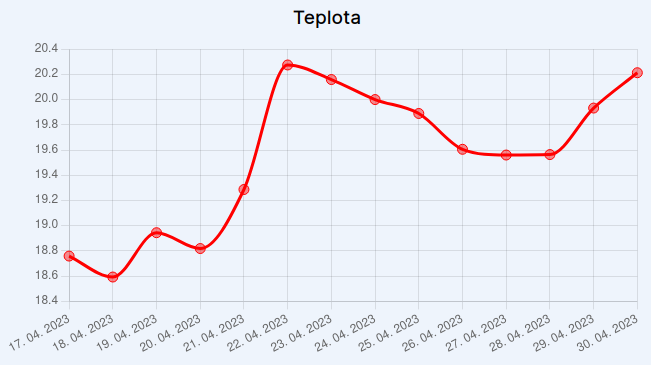
\includegraphics[width=0.6\textwidth]{images/graf.png}
    \caption{Graf s teplotami}
    \label{ukazka_grafu}
\end{figure}

\subsection{Mapa stanic}
Aby si mohl uživatel zobrazit data, musí se dostat na stránku s mapou, ve které je vidět bod. Po kliknutí na bod se dozví poslední naměřené údaje a může se prokliknout pomocí odkazu na podrobnější údaje v podobě grafů.

Pro vykreslení bodů do mapy jsme použili opensource knihovnu leaflet.js, která disponuje velkou škálou možností pro vykreslení bodů, množin a tvarů.
Avšak vybrání této knihovny také nebylo jednoduché. Prvoplánově jsme zamýšleli použít známé mapy jako jsou google maps nebo apple maps, ale implementace těchto knihoven byla pro naše účely zbytečně složitá. Dále tyto knihovny obsahují zdlouhavě a neintuitivní dokumentace, což je při práci s nimi nepříjemné.
Knihovna leaflet je populární a rozsáhle používána pro mobilní aplikace. Použití této mapy lze pozorovat například u dopravce české dráhy, sociální sítě Facebook a flickr.

\begin{figure}[h] %screenshot grafu 
    \centering
    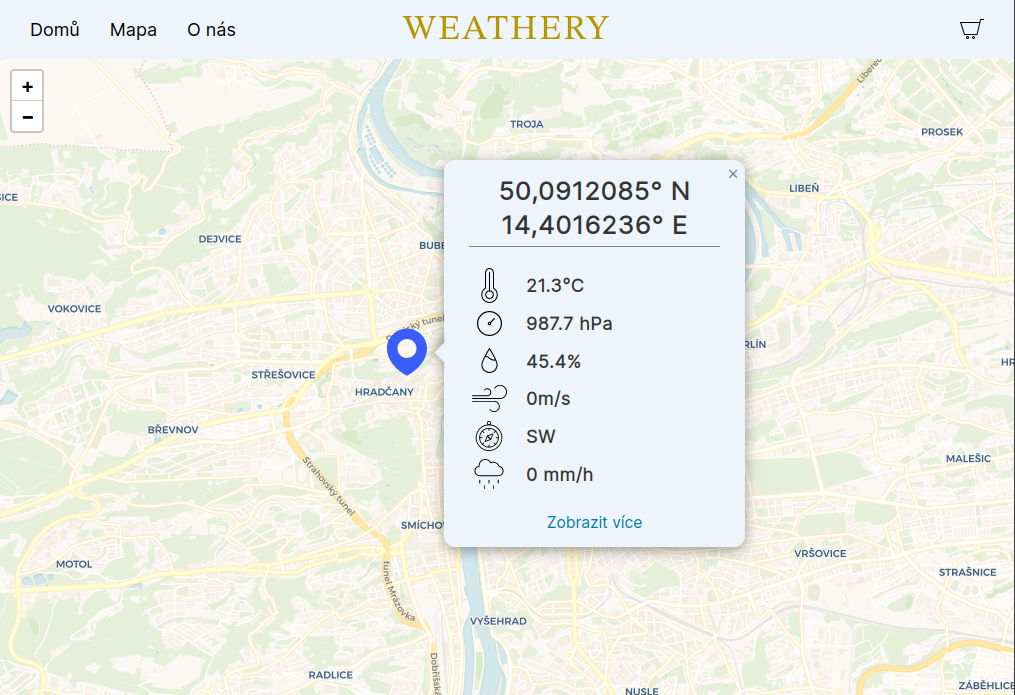
\includegraphics[width=0.6\textwidth]{images/mapa.png}
    \caption{Mapa stanic}
    \label{mapa}
\end{figure}


Pro nastavení mapy jsme zvolili světlé pozadí s málo kontrastním vykreslením vodních ploch, obytných oblastí, silnic, přírodních míst a hranic států. Uživatel má možnost libovolně mapu oddalovat a přibližovat, přičemž výchozím bodem mapy je Praha, na kterou je mapa po spuštění zaměřená.

\subsection{Design}
Design znamená vizuální podoba stránky.
Naším cílem bylo vytvořit intuitivní prostředí pro uživatele, ve kterém se dokáže rychle a jednoduše pohybovat.

Prvním setkáním s designem webu je domovská stránka, která obsahuje funkci detekující kolečko myši.
Právě tímto pohybem se stránka odhaluje a postupně mění. V průběhu animace se uživatel dozví informace o dlouhodobějších změnách počasí a srovnání počasí napříč roky.

%About us 
Na stránce nákup se uživatel dozví podobu stanice a je obeznámen s registrací a podrobnostmi.
\newpage
\begin{figure}[h] %screenshot grafu 
    \centering
    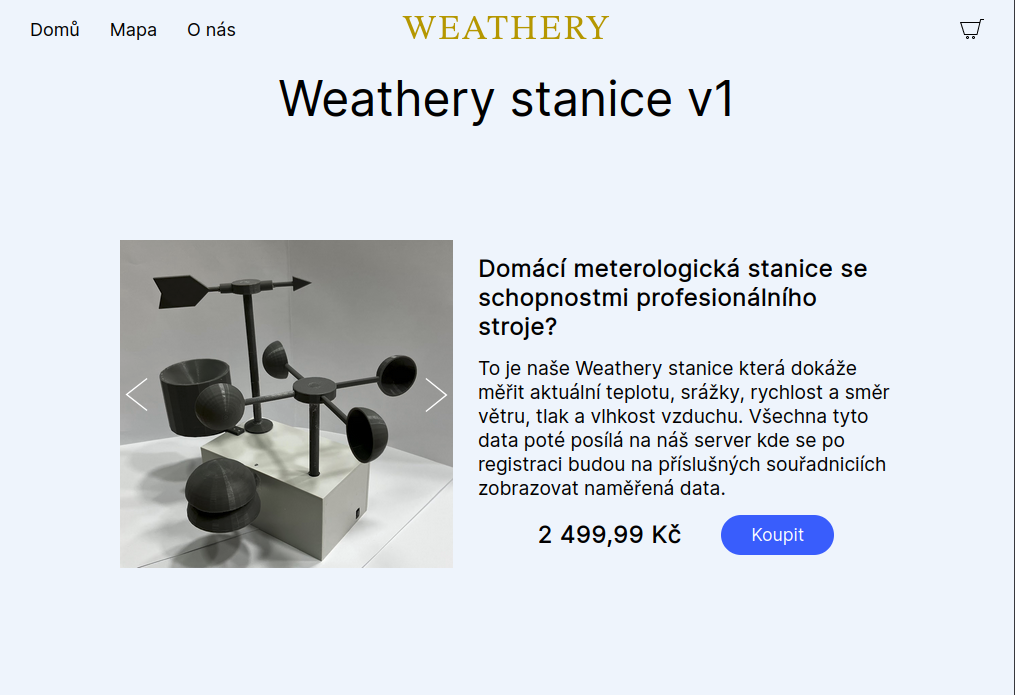
\includegraphics[width=0.6\textwidth]{images/nakup.png}
    \caption{Nákup stanice}
    \label{nakup}
\end{figure}


\newpage
\printbibliography
\listoffigures

\end{document}
